% !TeX root = ../thuthesis-example.tex

\chapter{服务器端高性能 \emph{insertRecords} 写入机制设计与实现}
经过客户端的预处理与 RPC 层的数据传输,写入请求最终会到达服务器端。服务器端对写入请求进行预处理后,交由存储引擎负责处理写入请求,并将这些数据最终持久化到磁盘上,服务器端的设计与实现对写入性能有至关重要的影响。如 \ref{sec:chap3-sec3-1} 中的实验结果所示,现有 IoTDB 服务器端对写入请求的处理有较大的性能瓶颈,不能满足高并发写入请求的需求。因此,本章将介绍对 \emph{insertRecords} 写入请求所设计的服务器端高性能写入机制。


\section{服务器端 \emph{insertRecords} 写入流程总览}
\ref{sec:chap3-sec2} 节介绍了 IoTDB 服务器端对 \emph{insertRecords} 写入请求执行的总体流程,新的执行流程和原有流程大体相似,单针对之前实验中发现的瓶颈,本工作进行了重新设计以优化写入性能。

\begin{figure}
  \centering
  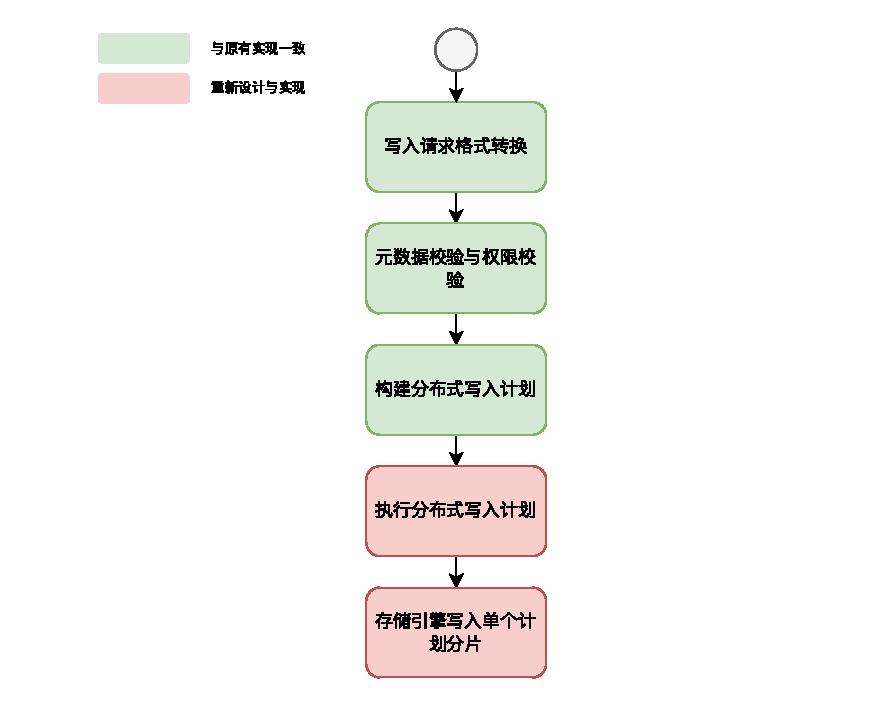
\includegraphics[width=0.9\linewidth]{new-storage-engine.pdf}
  \caption{服务器端 \emph{insertRecords} 写入流程}
  \label{fig:iotdb-insertRecords-flow}
\end{figure}

图 \ref{fig:iotdb-insertRecords-flow} 展示了 \emph{insertRecords} 写入请求到达 IoTDB 服务器端以后的总体执行流程,其中绿色部分代表这些流程与 IoTDB 原有设计基本保持一致,因为它们并不是写入的瓶颈所在;红色部分代表了在原有实现中存在的性能瓶颈,本工作对这些部分进行了重新设计与实现以提高写入性能。